% =============================================================================
% Section 5. The Energy Security Index
% Specification: R/indices/build_energy_security_index_v2.R, R/indices/index_builder_core.R,
% the ES theme builders in R/categories/** as called from scripts/10_build_themes.R,
% config/weights.yml (energy_security), config/missing_data.yml, config/rankability.yml,
% docs/methodology.md section 4. Results: paper/results/es.json, scripts/paper/fig_es.R (final
% rerun of 2026-10-12). Further results: Online Appendix (sections/oa_es.tex, oa:es);
% variable inventory: Appendix A.
% =============================================================================
\section{The Energy Security Index}\label{sec:es}\label{sec:energy_security}

The Energy Security pillar $\ES_{its}$ asks how far economy $i$ can rely on the supply of
technology $t$ at supply-chain stage $s$: of the minerals it is built from, of the materials,
components and equipment that embody it, and of the energy it delivers. Following
\citet{cherp2014concept}, security is the low vulnerability of vital energy systems, scored on the
dimensions the measurement literature shares: domestic resources, dependence on imports and on few
suppliers, price stability and access
\citep{kruyt2009indicators,sovacool2011conceptualizing,winzer2012conceptualizing,ang2015energy}; in
the terms of \citet{cherp2011three}, sovereignty, resilience and robustness. Because the ``fuel'' of
a clean technology is a bundle of minerals and manufactured inputs, the pillar borrows the
supply-risk logic of the criticality literature
\citep{graedel2012methodology,nassar2020evaluating,kowalski2023raw,iea2025gcmo} and the
concentration index of \citet{hirschman1945national}. A higher score means a more secure position;
the Strategic Index (Section~\ref{sec:strategic}) uses the need $1-\ES_{its}$.

% -----------------------------------------------------------------------------
\subsection{Construction}\label{subsec:es_aggregation}

Ten categories (Table~\ref{tab:es_structure}, weights summing to 42) are combined by the rules of
Section~\ref{sec:normalization} into the available-case weighted mean of
equation~\eqref{eq:pillar}. Registers of holders, producers, exporters or investors carry the zero
rule and the zero-anchored S-curve of equation~\eqref{eq:scurve_zero}, the other themes the
global-average rule (Table~\ref{tab:missing_rules}). The category bundle, and with it the effective
weights of equation~\eqref{eq:effective_weight}, differs across pairs but is common to all
economies within one. Mineral-level terms are aggregated to a technology with demand weights from
the IEA Critical Minerals Dataset \citep{iea2026cmdata}, Stated Policies scenario:
\begin{equation}\label{eq:es_demand_weights}
  w^{y}_{mt}=\frac{D^{y}_{mt}}{\sum_{t'}D^{y}_{mt'}},\qquad
  \tilde w^{y}_{mt}(M)=\frac{w^{y}_{mt}}{\sum_{m'\in M}w^{y}_{m't}},\qquad m\in M,
\end{equation}
where $D^{y}_{mt}$ is the demand for mineral $m$ from application $t$ in the base year $y_0=2025$
or the horizon $y_1=2035$, and $\tilde w$ renormalizes over the set $M$ of minerals a category
observes: $t$'s share of the mineral's clean-energy demand.

\begin{table}[tbp]
\centering
\begin{threeparttable}
\caption{Structure of the Energy Security pillar}
\label{tab:es_structure}
\scriptsize
\setlength{\tabcolsep}{3pt}
\begin{tabularx}{\textwidth}{@{}>{\raggedright\arraybackslash}p{2.1cm}
  >{\raggedright\arraybackslash}p{2.6cm}
  >{\raggedright\arraybackslash}X
  >{\raggedright\arraybackslash}p{2.6cm}
  >{\raggedright\arraybackslash}p{0.9cm}@{}}
\toprule
Category (weight) & Stages: technologies & Components & Sources & Rule\\
\midrule
Foreign Dependency (6) & Up, Mid: Bat, EV, Grid, H$_2$, Sol, Wind &
own share and $1-\HHI$ of mined (Up) or refined (Mid) mineral supply, 2025 and 2035; Mid: share
of world manufacturing capacity (Bat, Sol, Wind), regional EV position (EV) &
IEA Critical Minerals Dataset; IEA ETP; IEA Global EV Outlook & avg, zero\\
Energy Imports (4) & Up: Oil, Gas, Coal & production balance (EJ) and self-sufficiency &
EI Statistical Review; EIA & avg\\
Reserves (4) & Up: all but Geo; Down: Sol, Wind, Geo &
proved fossil reserves; demand-weighted mineral reserves; identified uranium resources;
renewable resource potential &
EI; USGS MCS 2026; Red Book; resource atlases & zero, avg\\
Trade (4) & Up, Mid: all but Geo, H$_2$ &
share of world basket exports; net basket imports/GDP; $1-$ world export
$\HHI^{\dagger}$ & Atlas; UN Comtrade; WDI & avg\\
Minerals Trade (4) & Up: Bat, EV, Grid, H$_2$, Sol, Wind &
demand-weighted share of world mineral exports; $1-\HHI^{\dagger}$ & UN Comtrade & zero\\
Production (6) & Up: Bat, EV, Grid, H$_2$, Sol, Wind, Nuc & demand-weighted mine production;
uranium mine output & EI; Red Book & zero\\
Energy Access (4) & Down: Coal, Oil, Gas, Sol, Wind, Nuc & energy supply per capita, level and
growth & EI & avg\\
Consumption (5) & Down: all but EV, Grid & installed capacity per capita, level and growth to 2035
& BNEF NEO 2024 & avg\\
Energy Prices (2) & Up: all but Geo & commodity price volatility$^{\dagger}$ & IMF PCPS & avg\\
Investment (3) & Up: Bat, EV; Mid: Bat, EV, Sol, Wind; Down: monitor technologies & investment,
momentum, operating and pipeline capacity & Clean Investment Monitor & zero\\
\bottomrule
\end{tabularx}
\begin{tablenotes}[flushleft]\footnotesize
\item \textit{Notes:} Weights from \texttt{config/weights.yml}, renormalized over the observed
categories of each cell (equation~\eqref{eq:pillar}). Up, Mid, Down: upstream, midstream,
downstream; Bat batteries, EV electric vehicles, Grid electric grid, H$_2$ green hydrogen, Sol
solar, Nuc nuclear, Geo geothermal. $^{\dagger}$Constant across economies within a pair. Rule:
missing-data rule of the themes (avg: global average; zero). Variables in
Appendix~\ref{app:variables}.
\end{tablenotes}
\end{threeparttable}
\end{table}

% -----------------------------------------------------------------------------
\subsection{Categories}\label{subsec:es_categories}

\paragraph{Foreign Dependency.}\label{subsec:es_fd} The core component is the economy's position in
the IEA's mined (upstream) and refined (midstream) supply of copper, cobalt, lithium, nickel,
graphite and the magnet rare earths. With $Q^{y}_{ims}$ the supply of mineral $m$ by economy $i$ at
stage $s$,
\begin{align}
  \sigma^{y}_{ims}&=\frac{Q^{y}_{ims}}{\sum_{j}Q^{y}_{jms}},\qquad
  \HHI^{y}_{ms}=\sum_{j}\big(\sigma^{y}_{jms}\big)^{2},\label{eq:es_fd_share}\\
  q_{imts}&=\tfrac14\Big(\Scurve^{0}[\sigma^{y_0}]_{s}+\Scurve^{0}[\sigma^{y_1}]_{s}
  +\Scurve[1-\HHI^{y_0}]_{s}+\Scurve[1-\HHI^{y_1}]_{s}\Big),\label{eq:es_fd_mineral}\\
  \mathrm{MS}_{its}&=\frac{\sum_{m}w^{y_1}_{mt}\,q_{imts}}{\sum_{m}w^{y_1}_{mt}}.
  \label{eq:es_fd_ms}
\end{align}
A non-supplier scores zero on the shares but keeps the concentration terms. Midstream, the
category adds the share of world manufacturing capacity including announced projects for
batteries, solar and wind \citep{iea2024etp}, over the world total including the source's residual
row, and four indices of the EV position of the economy's IEA region. The IEA reports the European
Union as one region, so every EU member carries the EU's 2035 share (0.15 in wind, 0.11 in
batteries, 0.00 in solar) and members are not ranked apart on it.

\paragraph{Energy Imports.}\label{subsec:es_imports} For oil, gas and coal upstream, with production
$P_{if}$ and consumption $C_{if}$ of fuel $f$ in exajoules,
\begin{equation}\label{eq:es_imports}
  B_{if}=P_{if}-C_{if},\qquad \beta_{if}=100\,\frac{P_{if}}{C_{if}},\qquad
  \mathrm{EI}_{if}=\tfrac12\Big(\Scurve[\beta]_{f}+\Scurve[B]_{f}\Big),
\end{equation}
the net balance and self-sufficiency, ranked within the fuel, from the Statistical Review for 2025
\citep{ei2026statistical}. Where it lists no production for an economy and fuel, production is
taken from the EIA's International Energy Statistics \citep{eia2026international}, counted as
observed and paired with consumption of the same year; Estonian coal, for which the Statistical
Review counts oil shale, remains missing.

\paragraph{Reserves.}\label{subsec:es_reserves} Upstream, the category ranks proved oil, gas and
coal reserves (end-2020, the last year the Energy Institute publishes them), reserves of nine
critical minerals from the USGS Mineral Commodity Summaries 2026 (end-2025, with the erratum that
puts Brazil's rare earths at 11\,Mt) \citep{usgs2026mcs}, and identified recoverable uranium
resources below USD 260/kgU from the OECD-NEA/IAEA Red Book \citep{oecdnea2026uranium}. With
$\rho_{im}$ the zero-anchored index of mineral $m$, zero for an unlisted holder,
\begin{equation}\label{eq:es_reserves}
  R_{it}=\Scurve^{0}\Big[\textstyle\sum_{m\in M_t}\tilde w^{y_0}_{mt}(M_t)\,\rho_{im}\Big]_{t},
\end{equation}
so a holder of one mineral does not score that mineral's rank for the whole technology. Holders
the USGS lists without a figure (not available, withheld or small) count as zero. Downstream, the
category scores solar, wind and geothermal resource potential.

\paragraph{Trade.}\label{subsec:es_trade} The crosswalk of Section~\ref{subsec:data_crosswalk}
assigns each pair a basket of HS six-digit products $G_{ts}$: nine midstream baskets and, upstream,
the raw materials of batteries, electric vehicles (battery-mineral ores and magnet rare earths), wind
(rare earths), solar (silicon metal), nuclear (uranium ores and natural uranium compounds), the
fossil fuels and the grid, whose basket holds copper and aluminium inputs rather than electricity.
The category is
\begin{equation}\label{eq:es_trade}
  c_{\mathrm{T},its}=\mean\Big\{\Scurve[-\HHI_{ts}],\
  \Scurve\Big[\tfrac{\sum_{h\in G_{ts}}X_{ih}}{\sum_{h\in G_{ts}}W_{h}}\Big]_{ts},\
  \Scurve\Big[-\tfrac{\sum_{h\in G_{ts}}(M_{ih}-X_{ih})}{\mathrm{GDP}_i}\Big]_{ts}\Big\}:
\end{equation}
the share of world basket exports and net basket imports relative to GDP, from the Atlas of
Economic Complexity \citep{growthlab2019trade,hausmann2014atlas} and WDI \citep{worldbank2026wdi},
and the concentration of world basket exports among UN Comtrade reporters in 2024
\citep{uncomtrade}, which excludes Hong Kong as a re-export hub and is ranked across the 18 basket
cells of the headline technologies. That term takes one value per pair, so it moves the pair's
level without reordering its economies.

\paragraph{Minerals Trade and Production.}\label{subsec:es_minerals_trade}\label{subsec:es_production}
Minerals Trade averages the demand-weighted zero-anchored shares of world exports of the
technology's minerals (for a non-reporter, partners' reported imports converted from CIF to FOB)
with a pair-constant concentration term. Production ranks mine output like reserves,
\begin{equation}\label{eq:es_production}
  \mathrm{P}_{it}=\Scurve^{0}\Big[\textstyle\sum_{m\in M_t}\tilde w^{y_0}_{mt}(M_t)\,\pi_{im}\Big]_{t},
\end{equation}
and, for nuclear, uranium mine output from the Red Book. Fossil output enters only through Energy
Imports.

\paragraph{Energy Access, Consumption, Prices and Investment.}\label{subsec:es_access}%
\label{subsec:es_consumption}\label{subsec:es_prices}\label{subsec:es_investment}
Downstream, Energy Access ranks energy supply per capita in 2025 and its growth since 2020, by
fuel; Consumption ranks installed capacity per capita in 2024 and its projected growth to 2035
\citep{bnef2024neo}. Both read a deeper, expanding domestic system as more secure; treating high
use as exposure would reverse the sign (Section~\ref{subsec:eo_shared}). Energy Prices is
$\Scurve[-\bar v_t]$, with $\bar v_t$ the mean annualized volatility of monthly log changes in the
technology's IMF commodity prices over 1, 5, 10 and 20 years \citep{imf2026pcps}, a world value.
Investment ranks clean-technology investment, its three-year momentum, and operating and pipeline
manufacturing capacity \citep{cim2026}; upstream critical-minerals investment is split between
batteries and electric vehicles by their IEA demand shares, 11.5 and 88.5 per cent.

% -----------------------------------------------------------------------------
\subsection{Results}\label{subsec:es_results}

\paragraph{Coverage.} The pillar scores 6{,}232 cells of the eleven headline technologies for 219
economies (195 sovereign, 24 territories) in 30 of the 33 pairs (Geothermal upstream and midstream
and Electric Grid downstream have no category). No pair is constant and no cell fully imputed; the
mean imputed weight share is 0.41, 0.23 and 0.27 by stage. All rankings and summaries use the 4{,}163 rankable cells
(Section~\ref{subsec:norm_diagnostics}): 1{,}124 of 2{,}181 upstream, where the world price series
places every economy in each pair while the mineral and fossil sources cover far fewer, 1{,}397 of
2{,}002 midstream and 1{,}642 of 2{,}049 downstream.

\paragraph{Distribution.} The median rankable cell scores 0.28 upstream (interquartile range 0.19
to 0.37), 0.46 midstream (0.36 to 0.53) and 0.44 downstream (0.35 to 0.52), with a right-skewed
upstream distribution (Figure~\ref{fig:es_distribution}): in the median upstream pair 71 per cent
of rankable economies score zero on Reserves and 84 per cent on Production. Technology-stage fixed
effects explain 44 per cent of the variance, country effects alone 12 per cent and both together
60 per cent (28 per cent of the within-pair variance), and the pair effects reflect the category
bundles rather than the cell-constant inputs. Rankings are meaningful within a pair; comparing one
economy's levels across pairs, as the Strategic Index does, mixes content with construction.

\begin{figure}[tbp]
  \centering
  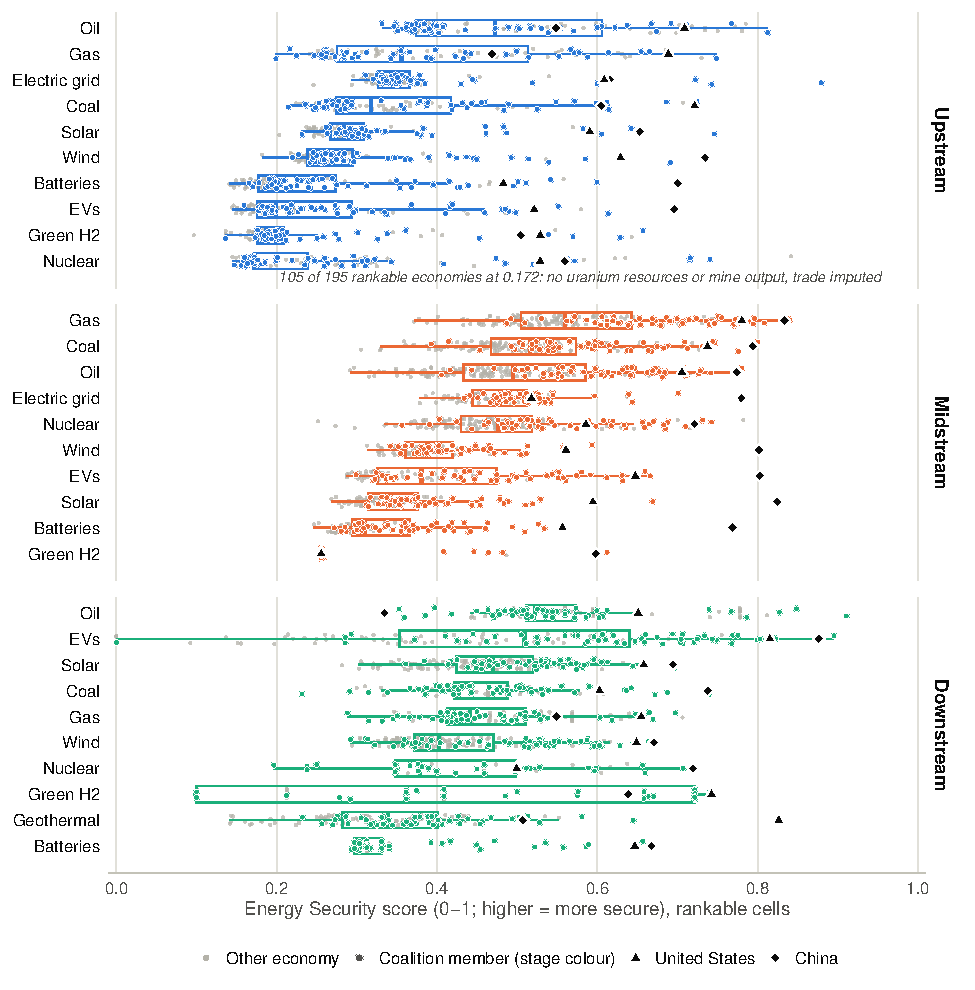
\includegraphics[width=\textwidth]{es_distribution}
  \caption{Energy Security by technology and stage, rankable cells (68 to 195 economies per
  pair; sovereign economy with at most half of the index weight imputed). Boxes span the
  interquartile range; gray dots are non-members, coloured dots coalition members in the stage
  colour; the triangle marks the United States and the diamond China. In Nuclear upstream, 105 of
  the 195 economies, which have neither uranium resources, production nor observed uranium trade,
  share the value 0.172 (Energy Prices plus an imputed Trade category). In Green Hydrogen
  midstream 90 per cent of economies share 0.26. Source: \texttt{energy\_security\_index} in
  \texttt{index\_outputs.rds}, final run; \texttt{scripts/paper/fig\_es.R}.}
  \label{fig:es_distribution}
\end{figure}

\paragraph{Drivers.} The exact category decomposition (equation~\eqref{eq:cat_decomp},
Figure~\ref{fig:es_category_contrib}) shows that upstream Trade supplies 31 per cent of the average
score, Energy Prices 20, Minerals Trade 16 and Foreign Dependency 13, while Reserves and Production
supply 7.2 and 3.1 per cent against mean effective weights of 20 and 19.5 per cent: for the typical
economy the registers add nothing, for the few holders they decide the top. Midstream, Trade
supplies 73 per cent and Foreign Dependency 26; downstream, Consumption 56 and Energy Access 24.
The cell-constant inputs carry a mean effective weight of 0.21 upstream and 0.22 midstream but
supply 36 and 26 per cent of the score. Reserves and Production correlate at a within-pair median
of 0.84, so upstream the pillar counts mineral endowment twice.

\begin{figure}[tbp]
  \centering
  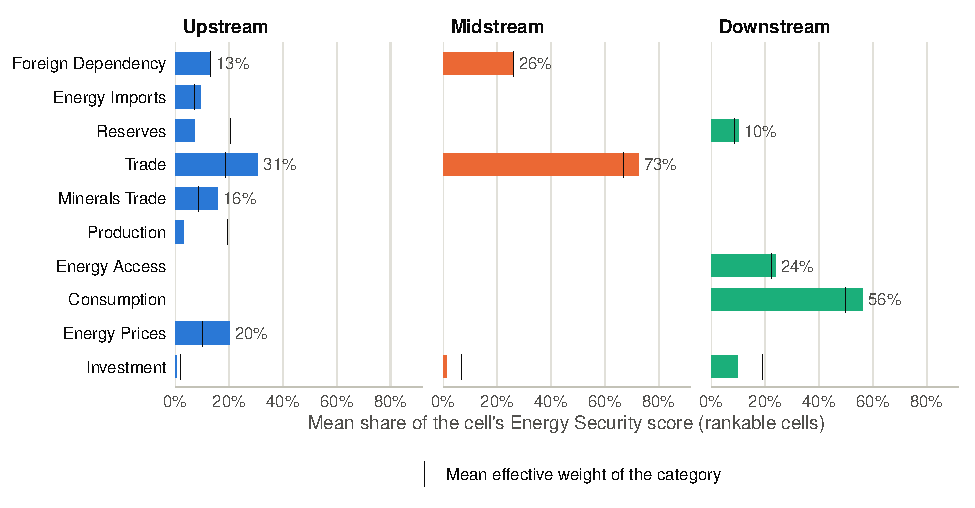
\includegraphics[width=\textwidth]{es_category_contrib}
  \caption{Average composition of Energy Security by stage, rankable cells. Bars: mean share of
  each category in the score, $\omega_{kits}c_{kits}/\ES_{its}$ (equation~\eqref{eq:cat_decomp});
  ticks: the category's mean effective weight. A bar much shorter than its tick, as for Reserves
  and Production upstream, marks a category on which most economies score zero. The upstream
  Energy Prices and Trade shares include Nuclear upstream (15 and 28 per cent without it). Sample:
  1{,}124 upstream, 1{,}397 midstream and 1{,}637 downstream cells. Source:
  \texttt{energy\_security\_outputs\$category\_contributions}; \texttt{scripts/paper/fig\_es.R}.}
  \label{fig:es_category_contrib}
\end{figure}

\paragraph{Uranium.} Nuclear upstream is scored on Energy Prices, Trade, Reserves and Production,
with effective weights of 1/8, 1/4, 1/4 and 3/8 (Figure~\ref{fig:es_nuclear_upstream}). Of the 195
rankable economies, 58 hold identified resources and 18 of them produce. The 105 economies with
neither and without observed uranium trade share one value, 0.172; the other 32 without uranium lie
between 0.145 and 0.201. Kazakhstan leads (0.84), ahead of Canada (0.74), Namibia and Australia
(0.72); China is tenth (0.56) and the United States eleventh (0.53); 31 of the 57 coalition members
hold resources. Read as a need, the common value becomes a uniform 0.83 that measures absence
rather than a gap domestic supply could close. Because 86 of the 174 countries with a Strategic
Index share it, the allied picks admit an upstream stage only where the country records reserves
or production of its resources (Section~\ref{subsec:si_allied}), a pick-eligibility rule, not part
of the index.

\begin{figure}[tbp]
  \centering
  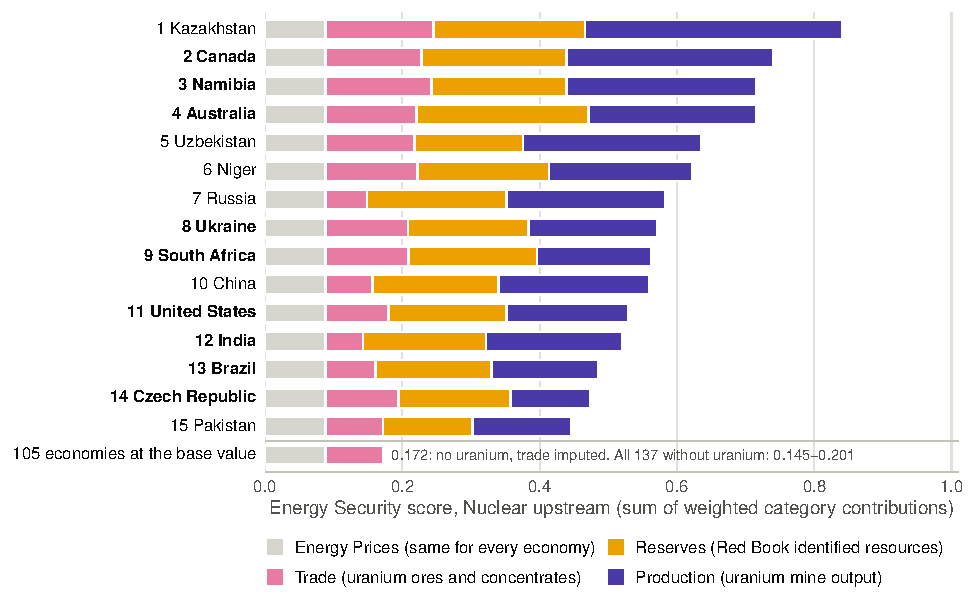
\includegraphics[width=\textwidth]{es_nuclear_upstream}
  \caption{Composition of Energy Security in Nuclear upstream: the 15 highest-ranked of 195
  rankable economies (coalition members in bold), split into Energy Prices (uranium price
  volatility, 0.088 for every economy), Trade (uranium ores, concentrates and natural uranium
  compounds), Reserves (identified resources below USD 260/kgU, OECD-NEA/IAEA Red Book) and
  Production (mine output). The bottom row stands for the 105 economies without uranium whose
  uranium trade is not observed (0.172). Source: \texttt{energy\_security\_index} and its category
  contributions; \texttt{scripts/paper/fig\_es.R}.}
  \label{fig:es_nuclear_upstream}
\end{figure}

\paragraph{Leaders and the coalition.} China leads 11 of the 30 pairs (Table~\ref{tab:es_leaders}):
three upstream mineral pairs, five midstream pairs, through its shares of refined supply and
manufacturing capacity \citep{iea2024etp,iea2025gcmo}, and three downstream pairs; no other
economy leads more than two. Upstream, leadership follows endowments (Saudi Arabia in oil, Qatar in
gas, Kazakhstan in nuclear, Chile in the grid and solar); in Oil upstream China ranks 34th, the
position of an importer (Figure~\ref{fig:es_top}). A coalition member is first in 16 pairs and in
the top three of all 30. The 57 members have mean within-pair percentiles of 0.59, 0.72 and 0.62 by
stage, against 0.47, 0.41 and 0.50 for other economies (Figure~\ref{fig:es_heatmap}); the United
States averages 0.95, China 0.92 (0.99 midstream), and Taiwan has the profile of a manufacturer
without resources (0.75 midstream, 0.01 upstream). Canada is the one high-income member with a
gap in the heatmap: its Downstream Consumption category is imputed at the global average in all
eight cells it enters, because the BloombergNEF outlook behind it neither models Canada nor has a
North American aggregate, so six of its nine scored Downstream cells are not rankable (the other
economies with the whole category imputed are Taiwan, Bermuda and seven South Asian economies). The
lead is unsurprising for a coalition of
large or resource-rich economies; whether members' strengths complement one another is the subject
of Section~\ref{sec:network}. Online Appendix~\ref{oa:es} details the leaders, the tiers and the
category correlations.

% Generated by scripts/paper/fig_es.R; do not edit by hand.
\begin{table}[tbp]
\centering
\begin{threeparttable}
\caption{Leading economies in each technology-stage pair of the Energy Security pillar (rankable cells)}
\label{tab:es_leaders}
\footnotesize
\begin{tabular}{@{}lrlllcrr@{}}
\toprule
Technology & $n$ & First & Second & Third & Best member (rank) & USA & CHN \\
\midrule
\multicolumn{8}{@{}l}{\textit{Upstream}}\\
Batteries & 106 & CHN 0.70 & AUS 0.60 & RUS 0.56 & AUS (2) & 9 & 1 \\
Coal & 96 & AUS 0.72 & USA 0.72 & RUS 0.71 & AUS (1) & 2 & 8 \\
Electric Grid & 106 & CHL 0.88 & COD 0.74 & PER 0.72 & CHL (1) & 5 & 4 \\
Electric Vehicles & 107 & CHN 0.70 & AUS 0.61 & RUS 0.58 & AUS (2) & 5 & 1 \\
Gas & 98 & QAT 0.75 & RUS 0.73 & USA 0.69 & QAT (1) & 3 & 33 \\
Green Hydrogen & 106 & ZAF 0.66 & RUS 0.64 & IDN 0.63 & ZAF (1) & 7 & 8 \\
Nuclear & 195 & KAZ 0.84 & CAN 0.74 & NAM 0.72 & CAN (2) & 11 & 10 \\
Oil & 97 & SAU 0.81 & VEN 0.79 & IRQ 0.78 & SAU (1) & 12 & 34 \\
Solar & 106 & CHL 0.75 & CHN 0.65 & PER 0.64 & CHL (1) & 5 & 2 \\
Wind & 107 & CHN 0.73 & AUS 0.69 & USA 0.63 & AUS (2) & 3 & 1 \\
\addlinespace
\multicolumn{8}{@{}l}{\textit{Midstream}}\\
Batteries & 106 & CHN 0.77 & USA 0.56 & CAN 0.53 & USA (2) & 2 & 1 \\
Coal & 190 & POL 0.80 & MOZ 0.80 & CHN 0.79 & POL (1) & 10 & 3 \\
Electric Grid & 106 & CHN 0.78 & JPN 0.70 & CHL 0.64 & JPN (2) & 22 & 1 \\
Electric Vehicles & 105 & CHN 0.80 & ESP 0.67 & HUN 0.66 & ESP (2) & 4 & 1 \\
Gas & 192 & KOR 0.84 & CHN 0.83 & ITA 0.81 & KOR (1) & 8 & 2 \\
Green Hydrogen & 106 & IDN 0.61 & CHN 0.60 & RUS 0.49 & IDN (1) & 12$^{95}$ & 2 \\
Nuclear & 188 & RUS 0.78 & FRA 0.74 & NLD 0.73 & FRA (2) & 30 & 5 \\
Oil & 192 & KOR 0.78 & CHN 0.77 & GAB 0.74 & KOR (1) & 11 & 2 \\
Solar & 106 & CHN 0.82 & IND 0.67 & USA 0.59 & IND (2) & 3 & 1 \\
Wind & 106 & CHN 0.80 & POL 0.59 & USA 0.56 & POL (2) & 3 & 1 \\
\addlinespace
\multicolumn{8}{@{}l}{\textit{Downstream}}\\
Batteries & 186 & CHN 0.67 & DEU 0.66 & USA 0.65 & DEU (2) & 3 & 1 \\
Coal & 186 & IDN 0.74 & CHN 0.74 & JPN 0.69 & IDN (1) & 9 & 2 \\
Electric Vehicles & 121 & TUR 0.90 & CHN 0.88 & VNM 0.82 & TUR (1) & 4 & 2 \\
Gas & 186 & KWT 0.71 & QAT 0.70 & KOR 0.67 & QAT (2) & 6 & 24 \\
Geothermal & 146 & USA 0.83 & IDN 0.64 & JPN 0.58 & USA (1) & 1 & 9 \\
Green Hydrogen & 186 & USA 0.74 & KOR 0.74 & ALB 0.72$^{49}$ & USA (1) & 1 & 63 \\
Nuclear & 68 & CHN 0.72 & FRA 0.71 & JPN 0.66 & FRA (2) & 17 & 1 \\
Oil & 186 & QAT 0.91 & OMN 0.85 & ARE 0.83 & QAT (1) & 23 & 186 \\
Solar & 191 & SAU 0.70 & AUS 0.70 & CHN 0.69 & SAU (1) & 4 & 3 \\
Wind & 186 & CHN 0.67 & CAN 0.66 & USA 0.65 & CAN (2) & 3 & 1 \\
\bottomrule
\end{tabular}
\begin{tablenotes}[flushleft]\footnotesize
\item \textit{Notes:} $\ES_{its}$ for the eleven headline technologies, final run. Only rankable cells enter: a sovereign economy with at most half of the cell's index weight imputed. Economies are identified by ISO3 code and followed by their score; $n$ is the number of rankable economies in the pair. ``Best member'' is the highest-ranked of the 57 coalition members, with its rank in parentheses; the USA and CHN columns give the ranks of the United States and China. A rank is one plus the number of rankable economies with a strictly higher score, so tied economies share a rank, and a superscript gives the number of economies that share it (the economy listed is the first of them alphabetically). Geothermal upstream, Geothermal midstream and Electric Grid downstream have no Energy Security score. Source: \texttt{energy\_security\_index} in \texttt{index\_outputs.rds}; \texttt{scripts/paper/fig\_es.R}.
\end{tablenotes}
\end{threeparttable}
\end{table}


\begin{figure}[tbp]
  \centering
  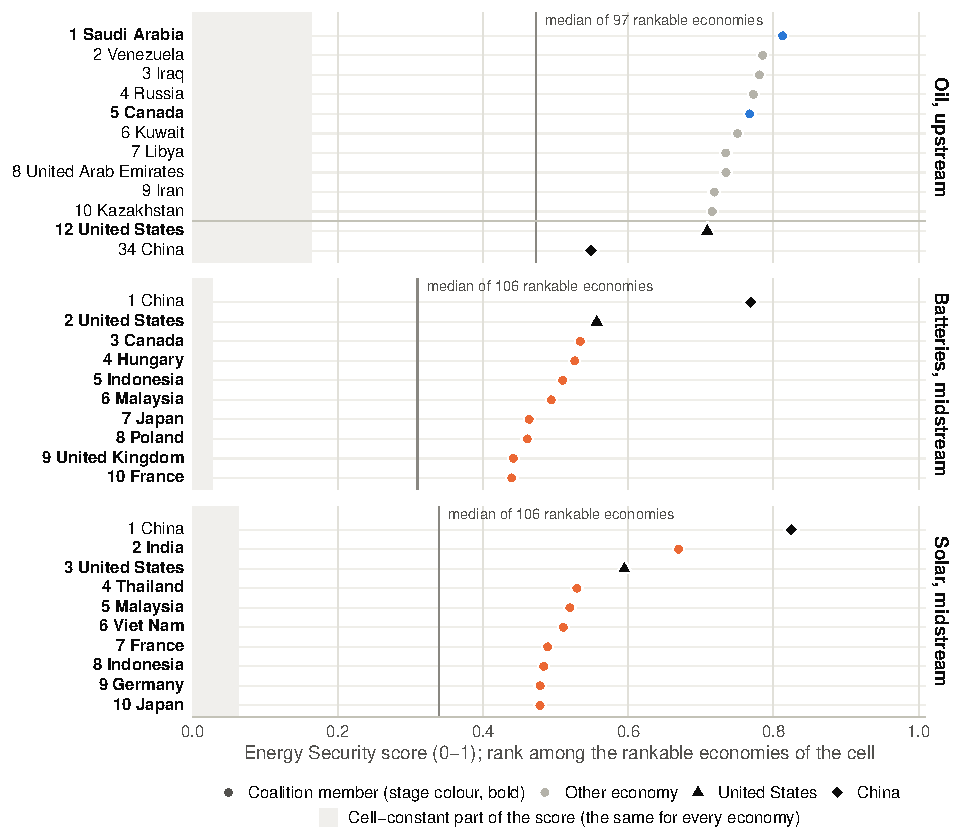
\includegraphics[width=\textwidth]{es_top}
  \caption{The ten highest-ranked economies in Oil upstream, Batteries midstream and Solar
  midstream (97, 106 and 106 rankable economies), with the United States (triangle) and China
  (diamond) appended when outside the top ten. Coalition members are in bold and the stage colour.
  The vertical line is the pair median; the shaded band is the cell-constant part of the score
  (0.16, 0.03 and 0.06). Source: \texttt{energy\_security\_index} and its variable contributions;
  \texttt{scripts/paper/fig\_es.R}.}
  \label{fig:es_top}
\end{figure}

\begin{figure}[tbp]
  \centering
  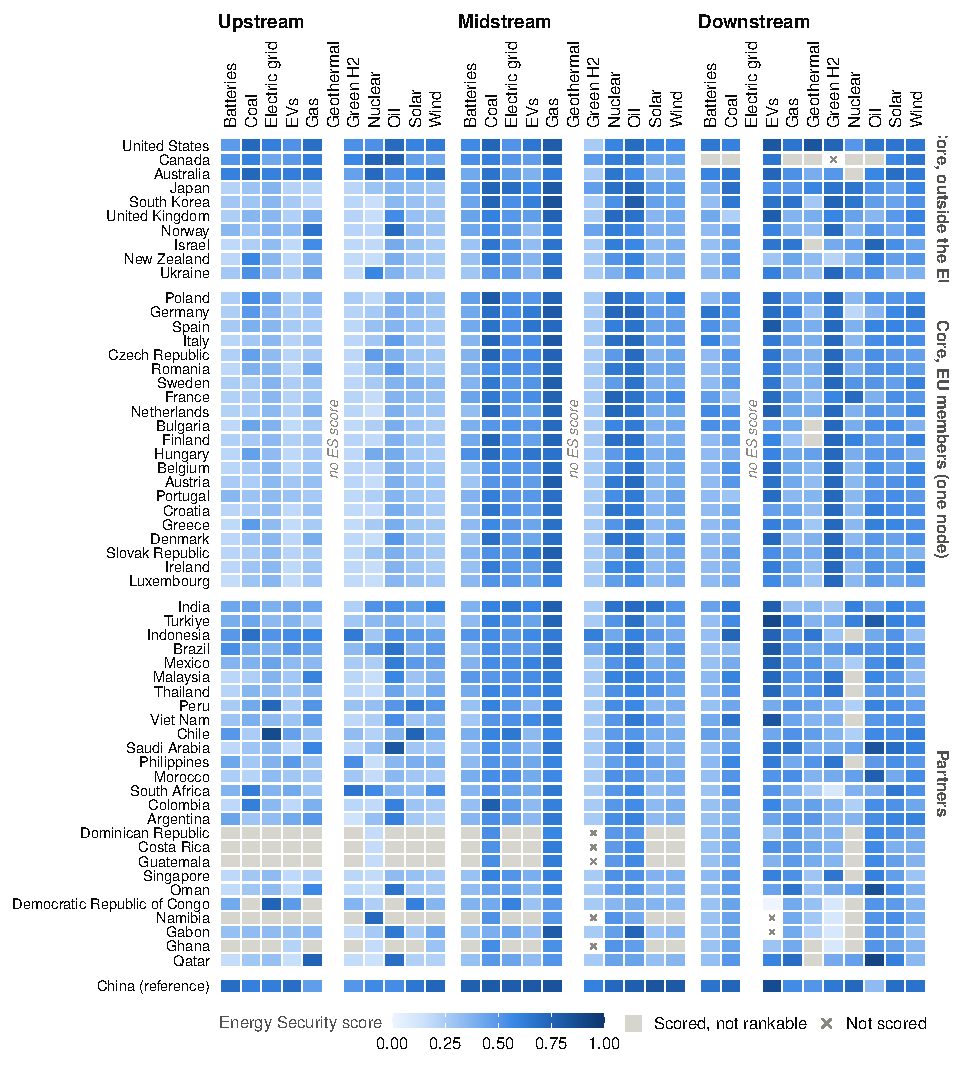
\includegraphics[width=\textwidth]{es_heatmap}
  \caption{Energy Security of the 57 coalition members across the 33 sectors, grouped into the
  ten core members outside the EU, the 21 core EU members and the
  26 partners, each ordered by mean within-pair percentile; China for reference. Colour gives
  $\ES_{its}$ for rankable cells; gray cells are scored but not rankable, crosses unscored, and the
  three sectors without an Energy Security score are blank. Canada's Downstream cells rest on an
  imputed Consumption category (its source, the BloombergNEF outlook, does not report Canada), so six
  of them are not rankable. Source: \texttt{energy\_security\_index}
  and \texttt{coalition\_members}; \texttt{scripts/paper/fig\_es.R}.}
  \label{fig:es_heatmap}
\end{figure}

\paragraph{Caveats.} Several pairs rank few distinct values: in the Strategic Index sample, Green
Hydrogen midstream has 34 of 40 countries at one value, Nuclear upstream 86 of 174, Green Hydrogen
downstream 45 of 158, Nuclear downstream 19 of 67 and Batteries downstream 38 of 138, and under the
need reading each mass point becomes a uniformly high need (Section~\ref{sec:strategic}).
Unquantified holders count as zero, and the downstream reading treats deeper domestic use of a
fossil fuel as security.
